% Figure from MATH 556 notes, section 40 (Baire category theorem: nested closed balls). Added, not from lecture.
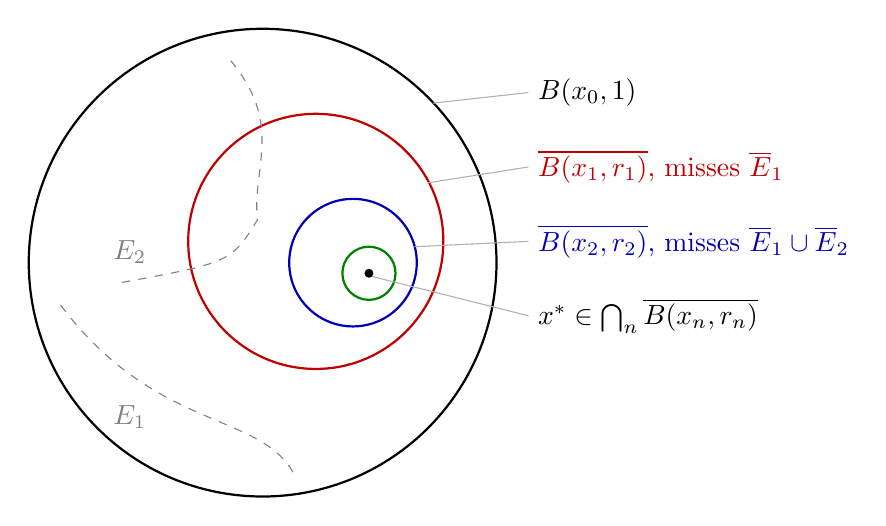
\begin{tikzpicture}[scale=1.35, >=stealth]
    \draw[thick] (0,0) circle (2.2);
    \draw[thick, red!75!black] (0.5,0.2) circle (1.2);
    \draw[thick, blue!70!black] (0.85,0.0) circle (0.6);
    \draw[thick, green!50!black] (1.0,-0.1) circle (0.25);
    \fill (1.0,-0.1) circle (1.2pt);
    \draw[gray, dashed] (-1.9,-0.4) .. controls (-1.0,-1.6) and (0.0,-1.4) .. (0.3,-2.0);
    \node[gray] at (-1.25,-1.45) {$E_1$};
    \draw[gray, dashed] (-0.3,1.9) .. controls (0.2,1.3) and (-0.1,0.9) .. (-0.05,0.4) .. controls (-0.3,0.0) .. (-1.4,-0.2);
    \node[gray] at (-1.25,0.1) {$E_2$};
    \node[anchor=west] at (2.5,1.6) {$B(x_0, 1)$};
    \draw[gray!60] (2.5,1.6) -- (1.6,1.5);
    \node[red!75!black, anchor=west] at (2.5,0.9) {$\overline{B(x_1, r_1)}$, misses $\overline{E}_1$};
    \draw[gray!60] (2.5,0.9) -- (1.55,0.75);
    \node[blue!70!black, anchor=west] at (2.5,0.2) {$\overline{B(x_2, r_2)}$, misses $\overline{E}_1 \cup \overline{E}_2$};
    \draw[gray!60] (2.5,0.2) -- (1.43,0.15);
    \node[anchor=west] at (2.5,-0.5) {$x^* \in \bigcap_n \overline{B(x_n, r_n)}$};
    \draw[gray!60] (2.5,-0.5) -- (1.03,-0.13);
\end{tikzpicture}
